\chapter{Implementation}

\section{Preprocessing}
\begin{itemize}
    \item data from \cref{sec:data-ana} is used for preprocessing
    \item Load data from the CSV files.
    \item Concatenate data from the first 10 lines of each file.
    \item Replace missing \acs{bssid} value
    \item Create a target variable.
    \item Normalize the data.
    \item Create sequences of data based on window_size.
    \item Encode the target variable.
    \item Split the data into training and testing sets.
\end{itemize}

\begin{figure}

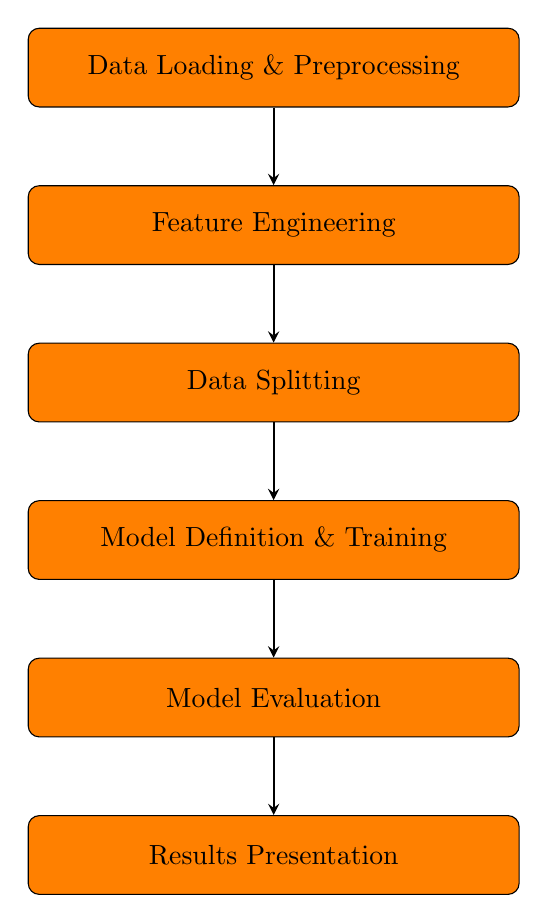
\begin{tikzpicture}
    % Define the styles for the processes and arrows
    \tikzstyle{process}=[rectangle, rounded corners, draw=black, fill=orange, text centered, text width=6cm, minimum height=1cm]
    \tikzstyle{arrow}=[thick,->,>=stealth]

    % Draw the processes
    \node[process] (data_loading) at (0, 0) {Data Loading \& Preprocessing};
    \node[process] (feature_engineering) at (0, -2) {Feature Engineering};
    \node[process] (data_splitting) at (0, -4) {Data Splitting};
    \node[process] (model_definition) at (0, -6) {Model Definition \& Training};
    \node[process] (model_evaluation) at (0, -8) {Model Evaluation};
    \node[process] (results_presentation) at (0, -10) {Results Presentation};

    % Draw the arrows between the processes
    \draw[arrow] (data_loading) -- (feature_engineering);
    \draw[arrow] (feature_engineering) -- (data_splitting);
    \draw[arrow] (data_splitting) -- (model_definition);
    \draw[arrow] (model_definition) -- (model_evaluation);
    \draw[arrow] (model_evaluation) -- (results_presentation);
\end{tikzpicture}

\caption{Flow diagram of the LSTM implementation process.}
\label{fig:flow_diagram}
\end{figure} 


\section{\ac{lstm}}
\begin{itemize}
    \item Decision in previous chapter for \ac{lstm}
    \item LSTM layer with 1000 units.
    \item Dense layer with softmax activation (number of units equal to the number of categories in the target variable).
\end{itemize}

\section{Training}

\begin{figure}
\begin{tikzpicture}[
    node distance=1cm and 1cm,
    mynode/.style={draw, rectangle, align=center, fill=blue!20, minimum width=3cm, minimum height=2cm},
    arrow/.style={->, >=stealth, shorten >=1pt, thick}
  ]
  
  % Data Preprocessing
  \node[mynode] (load) {Load Data};
  \node[mynode, below=of load] (concat) {Concatenate};
  \node[mynode, below=of concat] (replace) {Replace Missing Values};
  \node[mynode, below=of replace] (normalize) {Normalize};
  \node[mynode, below=of normalize] (sequence) {Create Sequences};
  \node[mynode, below=of sequence] (encode) {Encode Target};
  \node[mynode, below=of encode] (split) {Train-Test Split};
  \node[fit=(load) (split), draw, dashed, inner sep=8pt, label=above:{\textbf{Data Preprocessing}}] (preprocessing) {};
  
  % Model Architecture
  \node[mynode, right=2cm of split, yshift=2cm] (lstm) {LSTM Layer};
  \node[mynode, below=of lstm] (dense) {Dense Layer};
  \node[fit=(lstm) (dense), draw, dashed, inner sep=8pt, label=above:{\textbf{Model Architecture}}] (architecture) {};
  
  % Training & Evaluation
  \node[mynode, right=2cm of dense] (compile) {Compile Model};
  \node[mynode, below=of compile] (train) {Train Model};
  \node[mynode, below=of train] (predict) {Generate Predictions};
  \node[mynode, below=of predict] (evaluate) {Evaluate Accuracy};
  \node[fit=(compile) (evaluate), draw, dashed, inner sep=8pt, label=above:{\textbf{Training \& Evaluation}}] (training) {};
  
  % Arrows
  \draw[arrow] (load) -- (concat);
  \draw[arrow] (concat) -- (replace);
  \draw[arrow] (replace) -- (normalize);
  \draw[arrow] (normalize) -- (sequence);
  \draw[arrow] (sequence) -- (encode);
  \draw[arrow] (encode) -- (split);
  \draw[arrow] (split) -- (lstm);
  \draw[arrow] (lstm) -- (dense);
  \draw[arrow] (dense) -- (compile);
  \draw[arrow] (compile) -- (train);
  \draw[arrow] (train) -- (predict);
  \draw[arrow] (predict) -- (evaluate);
  
  \end{tikzpicture}
\caption{LSTM neural network architecture.}
\label{fig:lstm_architecture}
\end{figure}
    
    
%\noindent
